\documentclass{scrartcl}

\usepackage{tikz-timing}
\usepackage{graphicx}
\usepackage{tikz}
\usepackage{circuitikz}
\usepackage{xcolor}
\usetikzlibrary{shapes.symbols}

\usepackage{listings}
\lstset{
  basicstyle=\ttfamily\footnotesize,
  mathescape
}

\newcommand{\core}{AES-128 HPC }
\newcommand{\clk}{\ensuremath{\texttt{clk}}}
\newcommand{\rst}{\ensuremath{\texttt{syn\_rst}}}
\newcommand{\svrsInValid}{\ensuremath{\texttt{in\_valid}}}
\newcommand{\svrsInReady}{\ensuremath{\texttt{in\_ready}}}
\newcommand{\svrsPlaintext}{\ensuremath{\texttt{in\_shares\_plaintext}}}
\newcommand{\svrsKey}{\ensuremath{\texttt{in\_shares\_key}}}
\newcommand{\svrsCiphertext}{\ensuremath{\texttt{out\_shares\_ciphertext}}}
\newcommand{\svrsOutValid}{\ensuremath{\texttt{out\_valid}}}
\newcommand{\svrsOutReady}{\ensuremath{\texttt{out\_ready}}}
\newcommand{\svrsSeed}{\ensuremath{\texttt{in\_seed}}}
\newcommand{\svrsSeedValid}{\ensuremath{\texttt{in\_seed\_valid}}}
\newcommand{\svrsSeedReady}{\ensuremath{\texttt{in\_seed\_ready}}}

\newcommand{\topName}{\ensuremath{\texttt{aes\_enc128\_32bits\_hpc}}}
\newcommand{\topModAES}{\ensuremath{\texttt{MSKaes\_32bits\_core}}}
\newcommand{\topModPRNG}{\ensuremath{\texttt{prng\_top}}}
\newcommand{\topModReseedCtrl}{\ensuremath{\texttt{reseed\_controller}}}
\newcommand{\topModsvrsCtrl}{\ensuremath{\texttt{reseed\_controller}}}
\newcommand{\SB}{\ensuremath{\texttt{SubBytes}}}
\newcommand{\SR}{\ensuremath{\texttt{ShiftRows}}}
\newcommand{\MC}{\ensuremath{\texttt{MixColumns}}}
\newcommand{\AK}{\ensuremath{\texttt{AddRoundKey}}}

% Ports of AES core
\newcommand{\portAESInValid}{\ensuremath{\texttt{valid\_in}}}
\newcommand{\portAESInReady}{\ensuremath{\texttt{in\_ready}}}
\newcommand{\portAESInPlaintext}{\ensuremath{\texttt{sh\_plaintext}}}
\newcommand{\portAESInKey}{\ensuremath{\texttt{sh\_key}}}
\newcommand{\portAESbusy}{\ensuremath{\texttt{busy}}}
\newcommand{\portAESOutValid}{\ensuremath{\texttt{cipher\_valid}}}
\newcommand{\portAESOutReady}{\ensuremath{\texttt{out\_ready}}}
\newcommand{\portAESOutCipher}{\ensuremath{\texttt{sh\_ciphertext}}}
\newcommand{\portAESRnd}{\ensuremath{\texttt{rnd}}}
\newcommand{\portAESRndReady}{\ensuremath{\texttt{in\_rnd\_ready}}}

% Ports of PRNG 
\newcommand{\portPrngSeed}{\ensuremath{\texttt{in\_seed}}}
\newcommand{\portPrngStartReseed}{\ensuremath{\texttt{start\_reseed}}}
\newcommand{\portPrngOutReady}{\ensuremath{\texttt{out\_ready}}}
\newcommand{\portPrngOutValid}{\ensuremath{\texttt{out\_valid}}}
\newcommand{\portPrngOutRnd}{\ensuremath{\texttt{out\_rnd}}}
\newcommand{\portPrngBusy}{\ensuremath{\texttt{busy}}}

\newcommand{\triviumKey}{\ensuremath{\texttt{key}[79:0]}}
\newcommand{\triviumIV}{\ensuremath{\texttt{IV}[79:0]}}
\newcommand{\triviumInState}{\ensuremath{1 | 1 | 1 | 0^{112} | \triviumIV | 0^{13} | \triviumKey}}
\newcommand{\triviumOut}{\ensuremath{\texttt{stream}}}

% AES submodule
\newcommand{\modAESdpState}{\ensuremath{\texttt{MSKaes\_32bits\_state\_datapath}}}
\newcommand{\modAESdpKey}{\ensuremath{\texttt{MSKaes\_32bits\_key\_datapath}}}
\newcommand{\modAESsbox}{\ensuremath{\texttt{MSKSbox}}}

\newcommand{\AESsboxIn}{\ensuremath{\texttt{bytes\_to\_SB}}}
\newcommand{\AESsboxOut}{\ensuremath{\texttt{bytes\_from\_SB}}}
\newcommand{\AESsboxRnd}{\ensuremath{\texttt{rnd}}}
\newcommand{\AESsboxValidIn}{\ensuremath{\texttt{sbox\_valid\_in}}}
\newcommand{\AESsboxValidOut}{\ensuremath{\texttt{sbox\_valid\_out}}}
\newcommand{\AESsboxFeedKey}{\ensuremath{\texttt{feed\_sb\_key}}}
\newcommand{\AESFetchIn}{\ensuremath{\texttt{tap\_top\_input}}}

\newcommand{\AESdpStatePlaintext}{\ensuremath{\texttt{sh\_plaintext}}}
\newcommand{\AESdpStateFromSB}{\ensuremath{\texttt{sh\_4bytes\_from\_SB}}}
\newcommand{\AESdpStateFromKey}{\ensuremath{\texttt{sh\_4bytes\_from\_key}}}
\newcommand{\AESdpStateToSB}{\ensuremath{\texttt{sh\_4bytes\_to\_SB}}}
\newcommand{\AESdpStateCiphertext}{\ensuremath{\texttt{sh\_ciphertext}}}

\newcommand{\AESdpKeyKey}{\ensuremath{\texttt{sh\_key}}}
\newcommand{\AESdpKeyToSB}{\ensuremath{\texttt{sh\_4bytes\_rot\_to\_SB}}}
\newcommand{\AESdpKeyFromSB}{\ensuremath{\texttt{sh\_4bytes\_rot\_from\_SB}}}
\newcommand{\AESdpKeyToAK}{\ensuremath{\texttt{sh\_4bytes\_to\_AK}}}


% dpState internal
\newcommand{\dpStateModMC}{\ensuremath{\texttt{MC\_unit}}}
\newcommand{\dpStateByteToMC}{\ensuremath{\texttt{a}}}
\newcommand{\dpStateByteFromMC}{\ensuremath{\texttt{b}}}
\newcommand{\dpStateCtrlRouteMC}{\ensuremath{\texttt{route\_MC}}}
\newcommand{\dpStateCtrlRouteLoop}{\ensuremath{\texttt{loop}}}
\newcommand{\dpStateCtrlRouteIn}{\ensuremath{\texttt{init}}}
\newcommand{\dpStateCtrlEnable}{\ensuremath{\texttt{state\_enable}}}

% dpKey internal
\newcommand{\dpKeyCtrlInit}{\ensuremath{\texttt{init}}}
\newcommand{\dpKeyCtrlLoop}{\ensuremath{\texttt{loop}}}
\newcommand{\dpKeyCtrlRouteScan}{\ensuremath{\texttt{\dpKeyCtrlInit||\dpKeyCtrlLoop}}}
\newcommand{\dpKeyCtrlRouteInit}{\dpKeyCtrlInit}
\newcommand{\dpKeyCtrlRouteLoop}{\dpKeyCtrlLoop}
\newcommand{\dpKeyCtrlRouteFromSB}{\ensuremath{\texttt{from\_SB}}}
\newcommand{\dpKeyCtrlEnable}{\ensuremath{\texttt{KH\_enable}}}

%% Time only
\newcommand{\timeCnrRound}{\ensuremath{\texttt{cnt\_round}}}
\newcommand{\timeCnrCycle}{\ensuremath{\texttt{cnt\_fsm}}}
\newcommand{\timeCnrExecCycles}{\ensuremath{\texttt{cnt\_cycles}}}

%%% Pseudo code 
\newcommand{\pP}[1]{\ensuremath{\texttt{P}_{#1}}}
\newcommand{\pK}[1]{\ensuremath{\texttt{K}_{#1}}}
\newcommand{\pCt}[1]{\ensuremath{\texttt{C}_{#1}}}
\newcommand{\pS}[2]{\ensuremath{\texttt{S}_{#1}^{#2}}}
\newcommand{\pRK}[2]{\ensuremath{\texttt{RK}_{#1}^{#2}}}

\newcommand{\pSB}[2]{\ensuremath{\texttt{SB}_{#1}^{#2}}}
\newcommand{\pSR}[2]{\ensuremath{\texttt{SR}_{#1}^{#2}}}
\newcommand{\pMC}[2]{\ensuremath{\texttt{MC}_{#1}^{#2}}}
\newcommand{\pAK}[2]{\ensuremath{\texttt{AK}_{#1}^{#2}}}

\newcommand{\pR}[2]{\ensuremath{\texttt{R}_{#1}^{#2}}}
\newcommand{\pRSB}[2]{\ensuremath{\texttt{RSB}_{#1}^{#2}}}
\newcommand{\SW}[1]{\ensuremath{\texttt{SubWord}(#1)}}

\newcommand{\RCON}[1]{\ensuremath{\texttt{RCON}^{#1}}}


%% Pipe data routing font Size
\newcommand{\pipeFS}{\scriptsize}
\newcommand{\cDP}[1]{2D{\pipeFS #1}}
\newcommand{\NcDP}[2]{#2{2D}{\pipeFS #1}}

%% Pipeline dp Key
\newcommand{\dpKeyDFF}[1]{\ensuremath{\texttt{sh\_m\_key[#1]}}}

\newcommand{\timeStartdpKey}[1]{D{}\cDP{\pRK{#1}{i-1}}}
\newcommand{\timeFivedpKey}[4]{\NcDP{\pRK{#1}{i-1}}{1}\cDP{\pRK{#2}{i-1}}\cDP{\pRK{#3}{i-1}}\cDP{\pRK{#4}{i-1}}}
\newcommand{\timePartdpKey}[4]{\cDP{\pRK{#2}{i-1}}\cDP{\pRK{#3}{i-1}}\cDP{\pRK{#4}{i-1}}}
\newcommand{\timeStopdpKey}[2]{\NcDP{\pRK{#1}{i}}{1}\cDP{\pRK{#2}{i}}}

\newcommand{\timeMidIdpKey}[4]{\NcDP{\pRK{#1}{i}}{1}\cDP{\pRK{#2}{i}}\cDP{\pRK{#3}{i}}\cDP{\pRK{#4}{i}}}
\newcommand{\timeMidIIdpKey}[4]{\NcDP{\pRK{#1}{i-1}}{1}\cDP{\pRK{#2}{i-1}}\cDP{\pRK{#3}{i-1}}\cDP{\pRK{#4}{i}}}
\newcommand{\timeMidIIIdpKey}[4]{\NcDP{\pRK{#1}{i-1}}{1}\cDP{\pRK{#2}{i-1}}\cDP{\pRK{#3}{i}}\cDP{\pRK{#4}{i}}}
\newcommand{\timeMidIIIIdpKey}[4]{\NcDP{\pRK{#1}{i-1}}{1}\cDP{\pRK{#2}{i}}\cDP{\pRK{#3}{i}}\cDP{\pRK{#4}{i}}}

\newcommand{\timeLinedpKeyI}[4]{\timeStartdpKey{#4}\timeFivedpKey{#1}{#2}{#3}{#4}\timeMidIdpKey{#1}{#2}{#3}{#4}\timeStopdpKey{#1}{#2}}
\newcommand{\timeLinedpKeyII}[4]{\timeStartdpKey{#4}\timeFivedpKey{#1}{#2}{#3}{#4}\timeMidIIdpKey{#1}{#2}{#3}{#4}\timeStopdpKey{#1}{#2}}
\newcommand{\timeLinedpKeyIII}[4]{\timeStartdpKey{#4}\timeFivedpKey{#1}{#2}{#3}{#4}\timeMidIIIdpKey{#1}{#2}{#3}{#4}\timeStopdpKey{#1}{#2}}
\newcommand{\timeLinedpKeyIIII}[4]{\timeStartdpKey{#4}\timeFivedpKey{#1}{#2}{#3}{#4}\timeMidIIIIdpKey{#1}{#2}{#3}{#4}\timeStopdpKey{#1}{#2}}

%% Pipeline dp State
\newcommand{\dpStateDFF}[1]{\ensuremath{\texttt{sh\_reg\_out[#1]}}}

% Start
\newcommand{\timeStInterndpStateXII}[4]{D{}\cDP{\pMC{#3}{i-1}}\cDP{\pMC{#4}{i-1}}\cDP{\pMC{#1}{i-1}}\cDP{\pS{#2}{i}}\cDP{\pS{#3}{i}}\cDP{\pS{#4}{i}}\cDP{\pS{#1}{i}}}
\newcommand{\timeStInterndpStateXIII}[4]{D{}\cDP{\pMC{#3}{i-1}}\cDP{\pMC{#4}{i-1}}\cDP{\pMC{#1}{i-1}}\cDP{\pMC{#2}{i-1}}\cDP{\pS{#3}{i}}\cDP{\pS{#4}{i}}\cDP{\pS{#1}{i}}}
\newcommand{\timeStInterndpStateXIV}[4]{D{}\cDP{\pMC{#3}{i-1}}\cDP{\pMC{#4}{i-1}}\cDP{\pMC{#1}{i-1}}\cDP{\pMC{#2}{i-1}}\cDP{\pMC{#3}{i-1}}\cDP{\pS{#4}{i}}\cDP{\pS{#1}{i}}}
\newcommand{\timeStInterndpStateXV}[4]{D{}\cDP{\pMC{#3}{i-1}}\cDP{\pMC{#4}{i-1}}\cDP{\pMC{#1}{i-1}}\cDP{\pMC{#2}{i-1}}\cDP{\pMC{#3}{i-1}}\cDP{\pMC{#4}{i-1}}\cDP{\pS{#1}{i}}}

\newcommand{\timeStInterndpStateXI}[4]{D{}\cDP{\pMC{3}{i-1}}\cDP{\pMC{7}{i-1}}\cDP{\pMC{#1}{i-1}}\cDP{\pS{#2}{i}}\cDP{\pS{#3}{i}}\cDP{\pS{#4}{i}}\cDP{\pS{#1}{i}}}
\newcommand{\timeStInterndpStateX}[4]{D{}\cDP{\pMC{#3}{i-1}}\cDP{\pMC{#4}{i-1}}\cDP{\pMC{#1}{i-1}}\cDP{\pMC{#2}{i-1}}\cDP{\pMC{#3}{i-1}}\cDP{\pMC{#4}{i-1}}\cDP{\pS{#1}{i}}}
\newcommand{\timeStInterndpStateIX}[4]{D{}\cDP{\pMC{#3}{i-1}}\cDP{\pMC{#4}{i-1}}\cDP{\pMC{#1}{i-1}}\cDP{\pMC{#2}{i-1}}\cDP{\pMC{#3}{i-1}}\cDP{\pS{#4}{i}}\cDP{\pS{#1}{i}}}
\newcommand{\timeStInterndpStateVIII}[4]{D{}\cDP{\pMC{#3}{i-1}}\cDP{\pMC{#4}{i-1}}\cDP{\pMC{#1}{i-1}}\cDP{\pMC{#2}{i-1}}\cDP{\pS{#3}{i}}\cDP{\pS{#4}{i}}\cDP{\pS{#1}{i}}}

\newcommand{\timeStInterndpStateIV}[4]{D{}\cDP{\pS{#3}{i-1}}\cDP{\pMC{#4}{i-1}}\cDP{\pMC{#1}{i-1}}\cDP{\pMC{#2}{i-1}}\cDP{\pMC{#3}{i-1}}\cDP{\pS{#4}{i}}\cDP{\pS{#1}{i}}}
\newcommand{\timeStInterndpStateV}[4]{D{}\cDP{\pS{#3}{i-1}}\cDP{\pMC{#4}{i-1}}\cDP{\pMC{#1}{i-1}}\cDP{\pMC{#2}{i-1}}\cDP{\pMC{#3}{i-1}}\cDP{\pMC{#4}{i-1}}\cDP{\pS{#1}{i}}}
\newcommand{\timeStInterndpStateVI}[4]{D{}\cDP{\pS{#3}{i-1}}\cDP{\pMC{#4}{i-1}}\cDP{\pMC{#1}{i-1}}\cDP{\pS{#2}{i}}\cDP{\pS{#3}{i}}\cDP{\pS{#4}{i}}\cDP{\pS{#1}{i}}}
\newcommand{\timeStInterndpStateVII}[4]{D{}\cDP{\pS{#3}{i-1}}\cDP{\pMC{#4}{i-1}}\cDP{\pMC{#1}{i-1}}\cDP{\pMC{#2}{i-1}}\cDP{\pS{#3}{i}}\cDP{\pS{#4}{i}}\cDP{\pS{#1}{i}}}

\newcommand{\timeStInterndpStateIII}[4]{D{}\cDP{\pS{#3}{i-1}}\cDP{\pS{#4}{i-1}}\cDP{\pMC{#1}{i-1}}\cDP{\pMC{#2}{i-1}}\cDP{\pMC{#3}{i-1}}\cDP{\pS{#4}{i}}\cDP{\pS{#1}{i}}}
\newcommand{\timeStInterndpStateII}[4]{D{}\cDP{\pS{#3}{i-1}}\cDP{\pS{#4}{i-1}}\cDP{\pMC{#1}{i-1}}\cDP{\pMC{#2}{i-1}}\cDP{\pS{#3}{i}}\cDP{\pS{#4}{i}}\cDP{\pS{#1}{i}}}
\newcommand{\timeStInterndpStateI}[4]{D{}\cDP{\pS{#3}{i-1}}\cDP{\pS{#4}{i-1}}\cDP{\pMC{#1}{i-1}}\cDP{\pS{#2}{i}}\cDP{\pS{#3}{i}}\cDP{\pS{#4}{i}}\cDP{\pS{#1}{i}}}
\newcommand{\timeStInterndpStateZ}[4]{D{}\cDP{\pS{#3}{i-1}}\cDP{\pS{#4}{i-1}}\cDP{\pMC{#1}{i-1}}\cDP{\pMC{#2}{i-1}}\cDP{\pMC{#3}{i-1}}\cDP{\pMC{#4}{i-1}}\cDP{\pS{#1}{i}}}

% End 
\newcommand{\timeEndInterndpStateXII}[4]{\cDP{\pMC{#2}{i}}\cDP{\pMC{#3}{i}}\cDP{\pMC{#4}{i}}\cDP{\pMC{#1}{i}}\cDP{\pS{#2}{i+1}}}
\newcommand{\timeEndInterndpStateXIII}[4]{\cDP{\pMC{#2}{i}}\cDP{\pMC{#3}{i}}\cDP{\pMC{#4}{i}}\cDP{\pMC{#1}{i}}\cDP{\pMC{#2}{i}}}

\newcommand{\timeEndInterndpStateXI}[4]{\NcDP{\pS{#2}{i}}{1}\cDP{\pMC{#3}{i}}\cDP{\pMC{#4}{i}}\cDP{\pMC{#1}{i}}\cDP{\pS{#2}{i+1}}}
\newcommand{\timeEndInterndpStateX}[4]{\NcDP{\pS{#2}{i}}{1}\cDP{\pMC{#3}{i}}\cDP{\pMC{#4}{i}}\cDP{\pMC{#1}{i}}\cDP{\pMC{#2}{i}}}

\newcommand{\timeEndInterndpStateVII}[4]{\NcDP{\pS{#2}{i}}{1}\cDP{\pS{#3}{i}}\cDP{\pMC{#4}{i}}\cDP{\pMC{#1}{i}}\cDP{\pMC{#2}{i}}}
\newcommand{\timeEndInterndpStateVI}[4]{\NcDP{\pS{#2}{i}}{1}\cDP{\pS{#3}{i}}\cDP{\pMC{#4}{i}}\cDP{\pMC{#1}{i}}\cDP{\pS{#2}{i+1}}}

\newcommand{\timeEndInterndpStateIII}[4]{\NcDP{\pS{#2}{i}}{1}\cDP{\pS{#3}{i}}\cDP{\pS{#4}{i}}\cDP{\pMC{#1}{i}}\cDP{\pMC{#2}{i}}}
\newcommand{\timeEndInterndpStateI}[4]{\NcDP{\pS{#2}{i}}{1}\cDP{\pS{#3}{i}}\cDP{\pS{#4}{i}}\cDP{\pMC{#1}{i}}\cDP{\pS{#2}{i+1}}}

% Full line
\newcommand{\timeLinedpStateXII}[4]{\timeStInterndpStateXII{#1}{#2}{#3}{#4}\timeEndInterndpStateXII{#1}{#2}{#3}{#4}}
\newcommand{\timeLinedpStateXIII}[4]{\timeStInterndpStateXIII{#1}{#2}{#3}{#4}\timeEndInterndpStateXIII{#1}{#2}{#3}{#4}}
\newcommand{\timeLinedpStateXIV}[4]{\timeStInterndpStateXIV{#1}{#2}{#3}{#4}\timeEndInterndpStateXIII{#1}{#2}{#3}{#4}}
\newcommand{\timeLinedpStateXV}[4]{\timeStInterndpStateXV{#1}{#2}{#3}{#4}\timeEndInterndpStateXIII{#1}{#2}{#3}{#4}}

\newcommand{\timeLinedpStateVIII}[4]{\timeStInterndpStateVIII{#1}{#2}{#3}{#4}\timeEndInterndpStateX{#1}{#2}{#3}{#4}}
\newcommand{\timeLinedpStateIX}[4]{\timeStInterndpStateIX{#1}{#2}{#3}{#4}\timeEndInterndpStateX{#1}{#2}{#3}{#4}}
\newcommand{\timeLinedpStateX}[4]{\timeStInterndpStateX{#1}{#2}{#3}{#4}\timeEndInterndpStateX{#1}{#2}{#3}{#4}}
\newcommand{\timeLinedpStateXI}[4]{\timeStInterndpStateXI{#1}{#2}{#3}{#4}\timeEndInterndpStateXI{#1}{#2}{#3}{#4}}

\newcommand{\timeLinedpStateIV}[4]{\timeStInterndpStateIV{#1}{#2}{#3}{#4}\timeEndInterndpStateVII{#1}{#2}{#3}{#4}}
\newcommand{\timeLinedpStateV}[4]{\timeStInterndpStateV{#1}{#2}{#3}{#4}\timeEndInterndpStateVII{#1}{#2}{#3}{#4}}
\newcommand{\timeLinedpStateVI}[4]{\timeStInterndpStateVI{#1}{#2}{#3}{#4}\timeEndInterndpStateVI{#1}{#2}{#3}{#4}}
\newcommand{\timeLinedpStateVII}[4]{\timeStInterndpStateVII{#1}{#2}{#3}{#4}\timeEndInterndpStateVII{#1}{#2}{#3}{#4}}

\newcommand{\timeLinedpStateZ}[4]{\timeStInterndpStateZ{#1}{#2}{#3}{#4}\timeEndInterndpStateIII{#1}{#2}{#3}{#4}}
\newcommand{\timeLinedpStateI}[4]{\timeStInterndpStateI{#1}{#2}{#3}{#4}\timeEndInterndpStateI{#1}{#2}{#3}{#4}}
\newcommand{\timeLinedpStateII}[4]{\timeStInterndpStateII{#1}{#2}{#3}{#4}\timeEndInterndpStateIII{#1}{#2}{#3}{#4}}
\newcommand{\timeLinedpStateIII}[4]{\timeStInterndpStateIII{#1}{#2}{#3}{#4}\timeEndInterndpStateIII{#1}{#2}{#3}{#4}}

%% PRNG section
\newcommand{\NRNDBITS}{\ensuremath{\texttt{NRNDBITS}}}
\newcommand{\MULHPCRND}{\ensuremath{\texttt{MUL\_HPC2\_RND}}}
\newcommand{\NTRIVIUMS}{\ensuremath{\texttt{NTRIVIUMS}}}
\newcommand{\UNROLL}{\ensuremath{\texttt{UNROLL}}}
\newcommand{\MAXUNROLL}{\ensuremath{\texttt{PRNG\_MAX\_UNROLL}}}


\usepackage{pgf}

% Debug to print label to nodes
\newif\ifdebug
%\debugtrue
\debugfalse

%%%% CONFIG
\def\debugFontSize{\tiny}
%%%%


%% Debug node
% #1: test
% #2: position
\newcommand{\debugN}[2][]{
    \node at #2 {\ifdebug o \else \fi};
    \node [above] at #2 {\debugFontSize \ifdebug #1 \else \fi};
}

% Basic rectangle:
% #1: draw param
% #2: uid
% #3: center
% #4: width 
% #5: height
% #6: amount of nodes on W side
% #7: amount of nodes on E side
% #8: amount of nodes on N side
% #9: amount of nodes on S side
\newcommand{\rectangle}[9][]{
    \coordinate (#2/TL) at ($#3 + (-#4/2,#5/2)$);
    \coordinate (#2/TR) at ($#3 + (#4/2,#5/2)$);
    \coordinate (#2/BL) at ($#3 + (-#4/2,-#5/2)$);
    \coordinate (#2/BR) at ($#3 + (#4/2,-#5/2)$);
    \draw [#1] (#2/TL) -- (#2/TR)%
    -- (#2/BR) -- (#2/BL) -- (#2/TL); 
    % Draw the nodes on side W
    \foreach \xi in {1,...,#6}{
        \pgfmathsetmacro\offy{(#5)/(#6+1)}
        \pgfmathsetmacro\yval{\xi*\offy}
        \coordinate (#2/W\xi) at ($(#2/TL) - (0,\yval)$);
        \debugN[W\xi]{(#2/W\xi)}
    }
    % Draw the nodes on side E
    \foreach \xi in {1,...,#7}{
        \pgfmathsetmacro\offy{(#5)/(#7+1)}
        \pgfmathsetmacro\yval{\xi*\offy}
        \coordinate (#2/E\xi) at ($(#2/TR) - (0,\yval)$);
        \debugN[E\xi]{(#2/E\xi)}
    }
    % Draw the nodes on side N
    \foreach \xi in {1,...,#8}{
        \pgfmathsetmacro\offx{(#4)/(#8+1)}
        \pgfmathsetmacro\xval{\xi*\offx}
        \coordinate (#2/N\xi) at ($(#2/TL) + (\xval,0)$);
        \debugN[N\xi]{(#2/N\xi)}
    }
    % Draw the nodes on side S
    \foreach \xi in {1,...,#9}{
        \pgfmathsetmacro\offx{(#4)/(#9+1)}
        \pgfmathsetmacro\xval{\xi*\offx}
        \coordinate (#2/S\xi) at ($(#2/BL) + (\xval,0)$);
        \debugN[S\xi]{(#2/S\xi)}
    }
    %%%
    \coordinate (#2/center) at #3;
    \coordinate (#2/south) at ($#3 - (0,#5/2)$);
}

%% Rectangle from corner locations
% #1: draw param
% #2: uid
% #3: TR pos
% #4: BL pos
% #5: amount of nodes on W side
% #6: amount of nodes on E side
% #7: amount of nodes on N side
% #8: amount of nodes on S side
\newcommand{\rectangleC}[8][]{
    % Extract width/height from the corners
    \coordinate (sizerC) at ($#3-#4$); 
    % Define coordinate for remaining cornes
    \path let \p1=(sizerC) in coordinate (TL) at ($#4+(0,\y1)$);
    \path let \p1=(sizerC) in coordinate (BR) at ($#4+(\x1,0)$);
    % Draw the rectange
    \draw [#1] #3 |- #4 #3 -| #4;
    % Draw the node on side W
    \foreach \xi in {1,...,#5}{
        \pgfmathsetmacro\propL{\xi/(#5+1)}
        \coordinate (#2/W\xi) at ($(TL)!\propL!#4$);
        \debugN[W\xi]{(#2/W\xi)}
    }
    % Draw the node on side E
    \foreach \xi in {1,...,#6}{
        \pgfmathsetmacro\propL{\xi/(#6+1)}
        \coordinate (#2/E\xi) at ($#3!\propL!(BR)$);
        \debugN[E\xi]{(#2/E\xi)}
    }
    % Draw the node on side N
    \foreach \xi in {1,...,#7}{
        \pgfmathsetmacro\propL{\xi/(#7+1)}
        \coordinate (#2/N\xi) at ($(TL)!\propL!#3$);
        \debugN[N\xi]{(#2/N\xi)}
    }
    % Draw the node on side S
    \foreach \xi in {1,...,#8}{
        \pgfmathsetmacro\propL{\xi/(#8+1)}
        \coordinate (#2/S\xi) at ($#4!\propL!(BR)$);
        \debugN[S\xi]{(#2/S\xi)}
    }
    % Generate general coordinate
    \coordinate (#2/TL) at (TL);
    \coordinate (#2/TR) at #3;
    \coordinate (#2/BL) at #4;
    \coordinate (#2/BR) at (BR);
    \coordinate (#2/center) at ($#3!0.5!#4$);
    \coordinate (#2/south) at ($(#2/BL)!0.5!(#2/BR)$);
}

% Flip-Flop
% 1: draw style
% 2: id 
% 3: loc
% 4: width
% 5: height
\newcommand{\DFF}[5][]{
    % Draw a rectangle
    \rectangle[#1]{rect}{#3}{#4}{#5}{1}{1}{1}{1}
    % Draw the triangle
    \pgfmathsetmacro\baseT{(#4)/3}
    \pgfmathsetmacro\baseTd{\baseT/2}
    \pgfmathsetmacro\heightT{(#5)/7}
    \coordinate (TC0) at ($(rect/south) - (\baseTd,0)$);
    \coordinate (TC1) at ($(rect/south) + (\baseTd,0)$);
    \coordinate (TC2) at ($(rect/south) + (0,\heightT)$);
    \draw [#1] (TC0) -- (TC2) -- (TC1);
    \coordinate (#2/D) at (rect/W1);
    \coordinate (#2/Q) at (rect/E1);
    \coordinate (#2/center) at #3;
    \coordinate (#2/north) at (rect/N1);
}

% XOR
% 1: draw style
% 2: id
% 3: loc
% 4: radius
\newcommand{\XOR}[4][]{
    % Draw a circle    
    \draw [#1] #3 circle (#4);
    % Generate coordinate for th xor
    \coordinate (#2/north) at ($#3 + (0,#4)$);
    \coordinate (#2/south) at ($#3 + (0,-#4)$);
    \coordinate (#2/east) at ($#3 + (#4,0)$);
    \coordinate (#2/west) at ($#3 + (-#4,0)$);
    \draw [#1] (#2/north) -- (#2/south);
    \draw [#1] (#2/west) -- (#2/east);
}


%

\definecolor{colorIN}{RGB}{255,0,0}
\definecolor{colorOUT}{RGB}{0,0,255}
\definecolor{colorSEED}{RGB}{0,100,32}




\begin{document}


\subsection{Architecture of the $\modAESdpKey$ module}

\begin{figure}
    \centering
    \resizebox{\textwidth}{!}{
        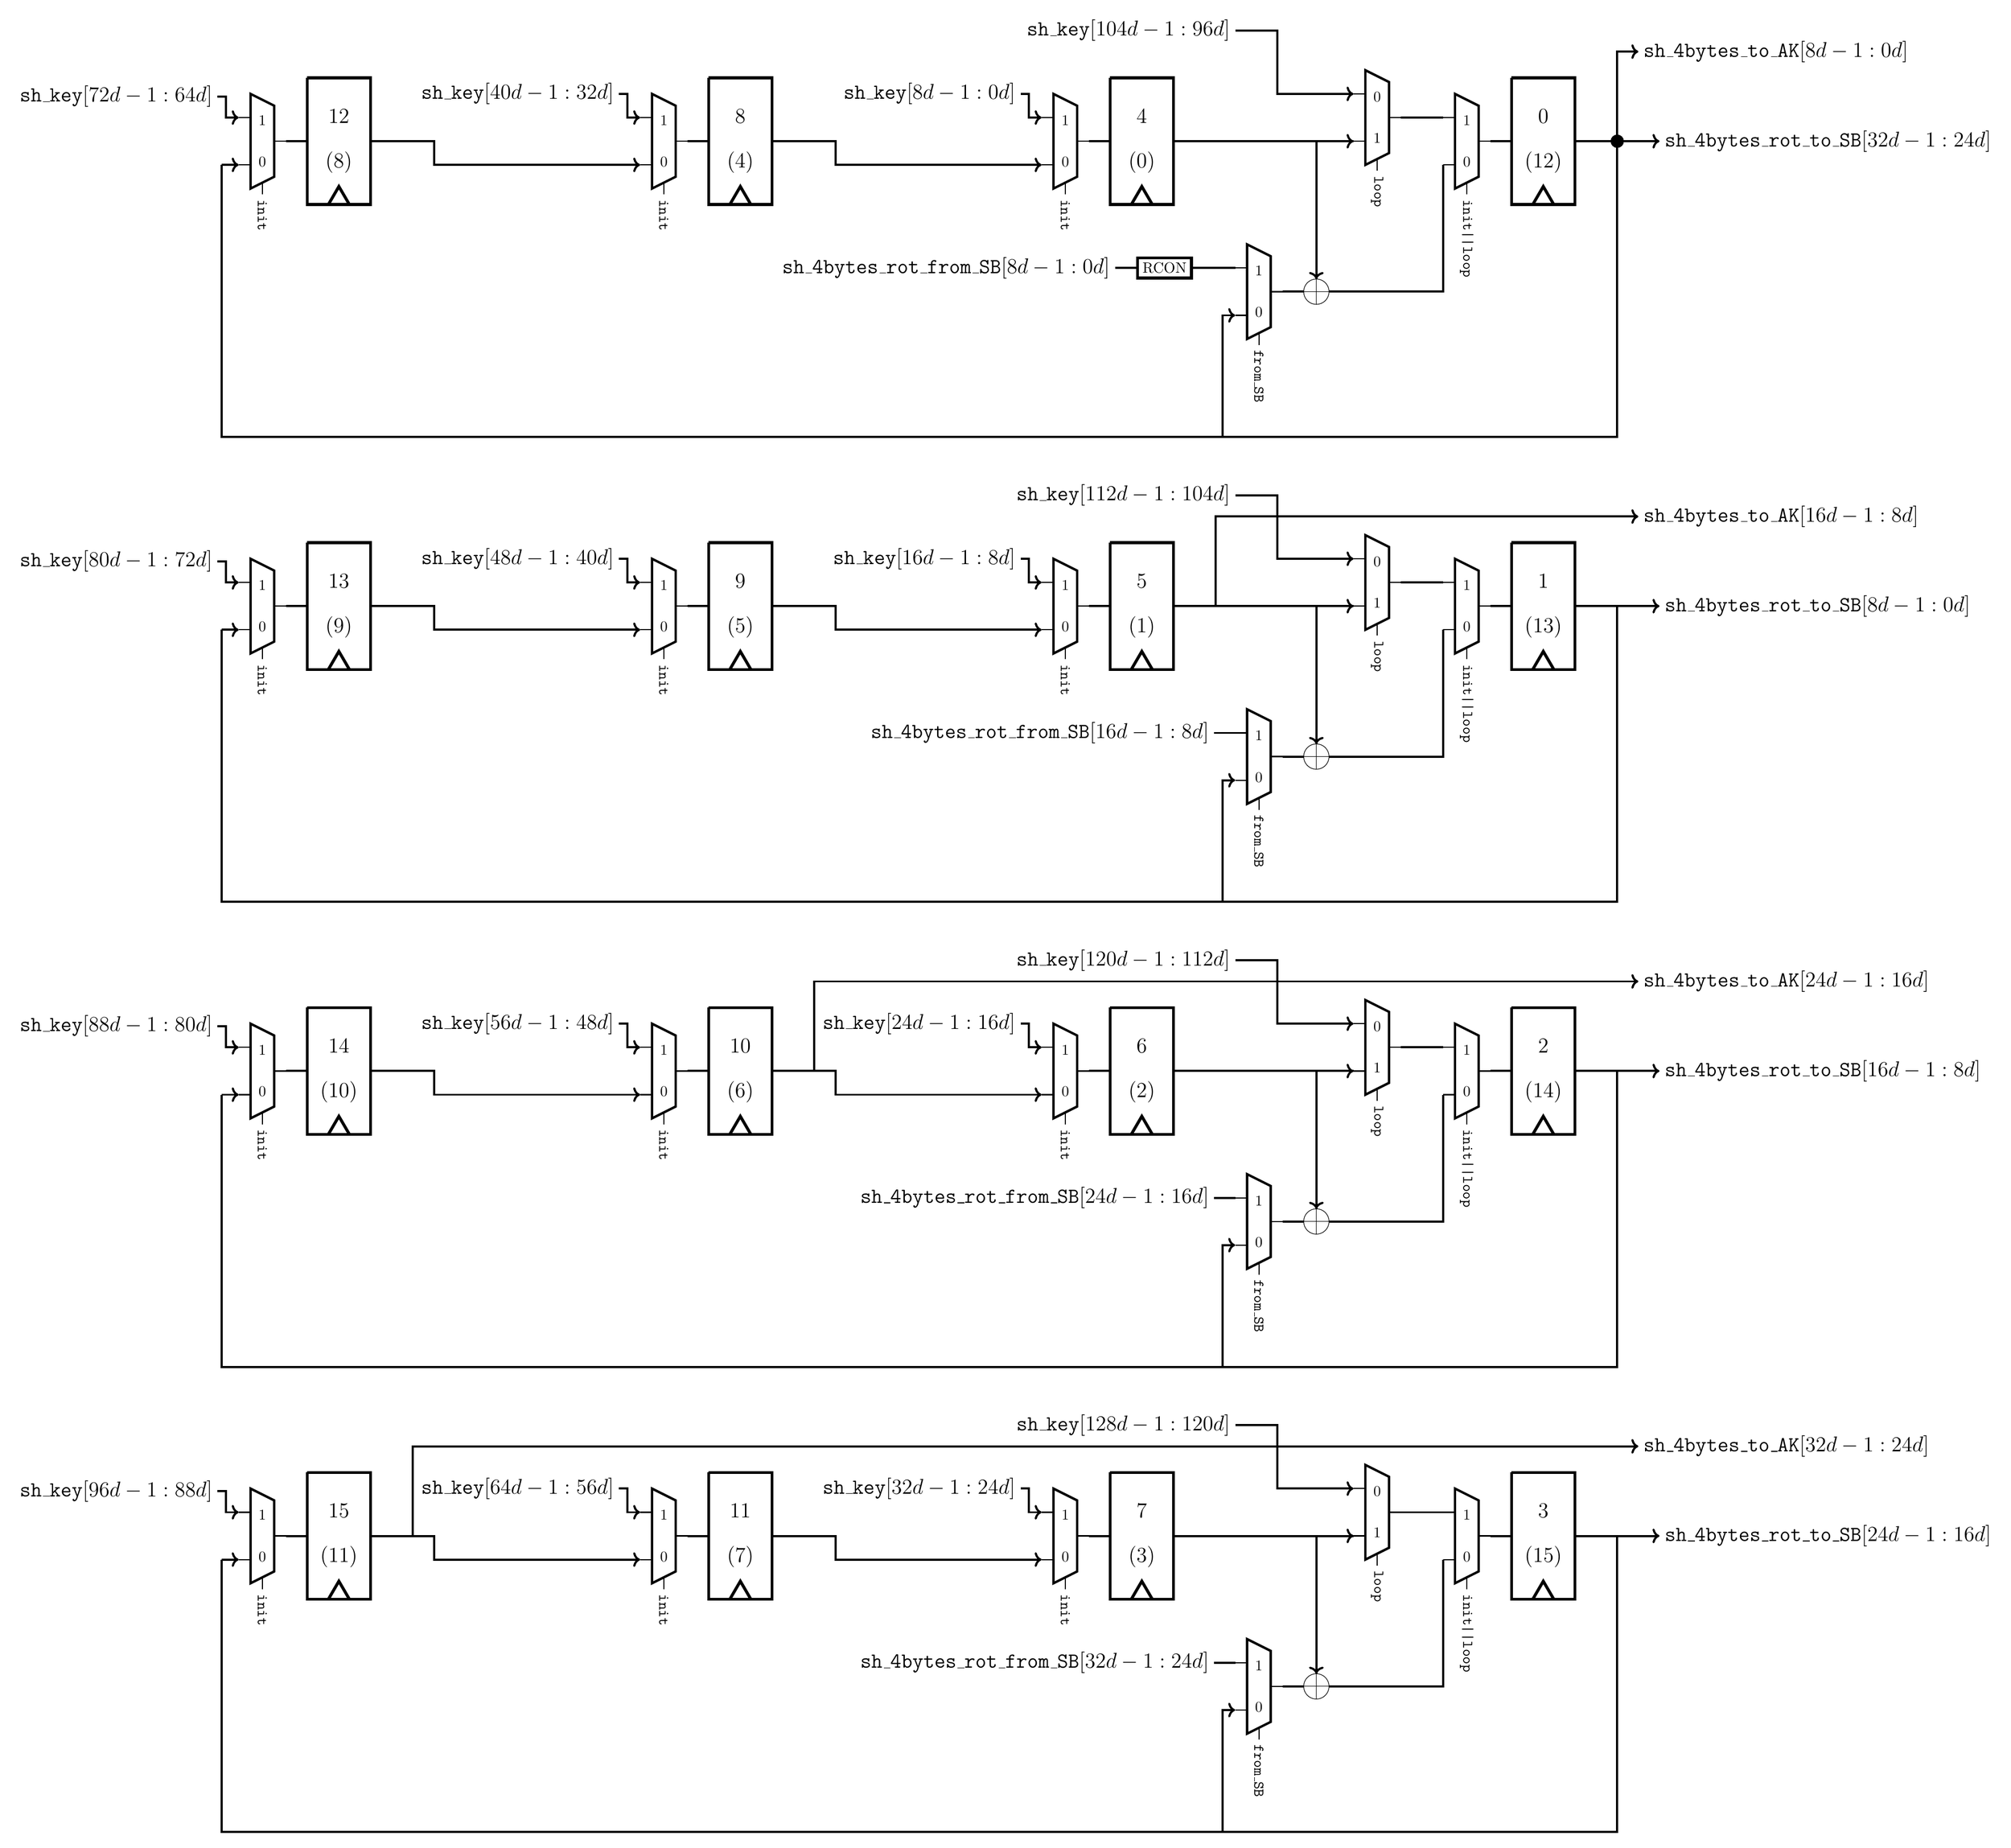
\begin{tikzpicture}
            % define a mux
\tikzset{mux2/.style={muxdemux,muxdemux def={Lh=4, NL=2, Rh=3,NB=1,w=1}}}

%% CONFIG
% Size of DFF instance
\def\widthDFF{1.5}
\def\heightDFF{3}
% Spacing between DFF instance
\def\spacexDFF{9.5}
\def\spaceyDFF{11}
% Y space for last column loop
\def\spaceyLoop{7}
% X space for last column input FIXME: modify to InFirstCol
\def\spacexInLastCol{1}
% Y space for for mux last column
\def\spaceyMuxInLastCol{0}
% Y-offset for XOR at the input for the  first column
\def\offsetyXorInFirstCol{3}

\def\fontS{\Large}
\def\fontCtrl{}

% Line width of DFF
\def\lwModule{0.7mm}
\def\lwWire{0.5mm}
\def\scaleCTIKZ{0.4}


%\debugtrue;

%% Macro for the ctrl signals of the mux2
% 1: mux_id
% 2: control sig
% 3: top value
% 4: bottom value
\newcommand{\muxCtrl}[4]{
    \node[anchor=west,rotate=270] at (#1.bpin 1) {\fontCtrl #2};
    \node at (#1.center up) {\fontCtrl #3};
    \node at (#1.center down) {\fontCtrl #4};
}


% Macro for a bloc with Register with mux input
% #1: style
% #2: id
% #3: loc (center DFF)
\newcommand{\DFFMUX}[3][]{
    % draw DFF
    \DFF[line width=\lwModule]{dffinst}{#3}{\widthDFF}{\heightDFF}
    % draw mux
    \node[line width=\scaleCTIKZ*\lwModule,mux2,anchor=rpin 1, xshift=-0.5cm] (#2/mux) at (dffinst/D) {}; 
    % Connector
    \draw[line width=\lwWire] (#2/mux.rpin 1) -- (dffinst/D);
    % draw small port at Q
    \coordinate (#2/out) at ($(dffinst/Q)+(1,0)$);
    \draw [line width=\lwWire] (dffinst/Q) -- (#2/out);
    % Generate remaining instance coordinate
    \coordinate (#2/text) at (dffinst/center);
    \coordinate (#2/in1) at (#2/mux.lpin 1);
    \coordinate (#2/in2) at (#2/mux.lpin 2);
    \coordinate (#2/north) at (dffinst/north);
    \coordinate (#2/ctrl) at (#2/mux.bpin 1);
    % Debug node
    \debugN[out]{(#2/out)}
    \debugN[in1]{(#2/in1)}
    \debugN[in2]{(#2/in2)}
    \debugN[text]{(#2/text)}
    \debugN[ctrl]{(#2/ctrl)}
}


%%%%% MAIN DRAWING %%%%%%%%%%%%%
\coordinate (D00) at (0,0);

% Draw all the DFFMUX instances
\foreach \xi in {0,...,3} {
    \foreach \yi in {0,...,3} {
        \pgfmathsetmacro\xshDFF{\spacexDFF*\xi}
        \pgfmathsetmacro\yshDFF{\spaceyDFF*\yi}
        \pgfmathsetmacro\DFFindex{int(12-4*\xi+\yi)}
        \DFFMUX{D\DFFindex}{($(D00)+(\xshDFF,-\yshDFF)$)}
        % Compute byte index
        \pgfmathsetmacro\DFFinitIndex{int(mod(16+\DFFindex-4,16))}
        \node [text width=1cm, align=center] at (D\DFFindex/text) {\Large $\DFFindex$ \\ \hfill \\ $(\DFFinitIndex)$};
        % Add the text to the DFF input
        \pgfmathsetmacro\mBound{int(8*\DFFindex)}
        \pgfmathsetmacro\MBound{int(8*(1+\DFFindex))}
    }
}

%%%% Generate the input construction at the first column 
\foreach \xi in {0,...,3}{
    % Draw the input mux
    \path let \p1=(D\xi/in1), \p2=(D\xi/north) in coordinate (locm) at ($(\x1,\y1)+(-1,\spaceyMuxInLastCol)$);
    \node[mux2,line width=\scaleCTIKZ*\lwModule,anchor=rpin 1] (MI\xi) at (locm) {};
    \draw [line width=\lwWire] (MI\xi.rpin 1) |- (D\xi/in1);
    % Create control signal for MUXin
    \muxCtrl{D\xi/mux}{$\dpKeyCtrlRouteScan$}{1}{0}
    \muxCtrl{MI\xi}{$\dpKeyCtrlRouteLoop$}{0}{1}
    % XOR
    \XOR{xor\xi}{($(D\xi/in2)+(-3,-\offsetyXorInFirstCol)$)}{0.3}
    \draw [line width=\lwWire] (xor\xi/east) -| (D\xi/in2);
    % Mux at the input of the XOR
    \node[mux2,line width=\scaleCTIKZ*\lwModule,anchor=rpin 1,xshift=-0.5cm] (MX\xi) at (xor\xi/west) {};
    \draw [line width=\lwWire] (MX\xi.rpin 1) -- (xor\xi/west);
    % Draw the ctrl of the mux
    \muxCtrl{MX\xi}{$\dpKeyCtrlRouteFromSB$}{1}{0}
    % Draw the feedback from the register
    \draw [->, line width=\lwWire] (D\xi/out) -- ++(0,-\spaceyLoop) -| ($(MX\xi.lpin 2)+(-0.3,0)$) -- (MX\xi.lpin 2);
    %% Generate feedback port 
    \draw [->,line width=\lwWire] (xor\xi/north) |- (MI\xi.lpin 2);
    \draw [->,line width=\lwWire] (MI\xi.lpin 2) -| (xor\xi/north);
    % Generate the coordinate of the ports
    \path let \p1=(MI\xi.lpin 2), \p2=(xor\xi/north) in coordinate (FB\xi) at (\x2,\y1);
    \debugN[FB\xi]{(FB\xi)}
    %% Generate key input
    \path let \p1=(MX\xi.lpin 1), \p2=(MI\xi.lpin 1) in coordinate (inKey\xi) at ($(\x1,\y2)+(0,1.5)$);
    \debugN[inKey\xi]{(inKey\xi)}
    \draw [->,line width=\lwWire] (inKey\xi) -- ++(1,0) |- (MI\xi.lpin 1);
    %% Generate Sbox input
    \coordinate (fromSB\xi) at (MX\xi.lpin 1); 
    \debugN[fromSB\xi]{(fromSB\xi)}
    %% Generate feedback loop
    \pgfmathsetmacro\rIdx{int(\xi+4)}
    \draw [line width=\lwWire] (D\rIdx/out) -- (FB\xi);
    %% Draw input nodes
    % to Sbox
    \coordinate (toSB\xi) at ($(D\xi/out)+(1,0)$);
    \debugN[toSB\xi]{(toSB\xi)}
    % to AK
    \pgfmathsetmacro\idxAK{int(\xi)}
    \path let \p1=(D\idxAK/out), \p2=(MI\xi.lpin 1) in coordinate (LocToAK\idxAK) at ($(\x1,\y2)+(0.5,1)$);
    \coordinate (toAK\idxAK) at (LocToAK\idxAK);
    \debugN[toAK\idxAK]{(toAK\idxAK)}
    % Key in 
    \pgfmathsetmacro\corrXI{int(mod(\xi+12,16))}
    \pgfmathsetmacro\mB{int((\corrXI)*8))}
    \pgfmathsetmacro\MB{int((\corrXI+1)*8)}
    \node [anchor=east] at (inKey\xi) {\fontS $\AESdpKeyKey[\MB d-1: \mB d]$};
}

%% Draw the port to SB
\node [anchor=west] at (toSB0) {\fontS $\AESdpKeyToSB[32d-1:24d]$};
\node [anchor=west] at (toSB1) {\fontS $\AESdpKeyToSB[8d-1:0d]$};
\node [anchor=west] at (toSB2) {\fontS $\AESdpKeyToSB[16d-1:8d]$};
\node [anchor=west] at (toSB3) {\fontS $\AESdpKeyToSB[24d-1:16d]$};
\draw [->,line width=\lwWire] (D0/out) |- (toSB0);
\draw [->,line width=\lwWire] (D1/out) |- (toSB1);
\draw [->,line width=\lwWire] (D2/out) |- (toSB2);
\draw [->,line width=\lwWire] (D3/out) |- (toSB3);

%%% Generate the inport port for columns other than first ones
%%% Generate also input connexions for the DFF units
\foreach \xi in {0,...,3}{
    \foreach \yi in {1,...,2}{
        % Fetch y coordinate of the input mux of first column
        \pgfmathsetmacro\refIdx{int(\xi)}
        \pgfmathsetmacro\DIdx{int(\xi+4*\yi)}
        \coordinate (refP) at (MI\refIdx.lpin 1);
        \path let \p1=(refP), \p2=(D\DIdx/in1) in coordinate (inKey\DIdx) at ($(\x2,\y1) + (-0.5,0)$);  
        \debugN[inKey\DIdx]{(inKey\DIdx)}
        \draw [->,line width=\lwWire] (inKey\DIdx) -- ++(0.2,0) |- (D\DIdx/in1);
        %% Input connexion
        \pgfmathsetmacro\DIdxp{int(\xi+4*(\yi+1))}
        \draw [->,line width=\lwWire] (D\DIdxp/out) -- ++(0.5,0) |- (D\DIdx/in2);
        %% Draw input port
        \pgfmathsetmacro\corrDIdx{int(mod(12+\DIdx,16))}
        \pgfmathsetmacro\mB{int(8*\corrDIdx)}
        \pgfmathsetmacro\MB{int(8*(\corrDIdx+1))}
        \node [anchor=east] at (inKey\DIdx) {\fontS $\AESdpKeyKey[\MB d-1:\mB d]$};
        %% Draw mux ctrl
        \muxCtrl{D\DIdx/mux}{$\dpKeyCtrlRouteInit$}{1}{0}
    }
}

%%% Generate input for the first column
\node [line width=\lwModule,rectangle,draw,anchor=east] (RCON) at ($(fromSB0)+(-\spacexInLastCol,0)$) {RCON};
\node [anchor=east,xshift=-0.5cm] (fSB0) at (RCON.west) {\fontS $\AESdpKeyFromSB[8d-1:0d]$};
\draw [line width=\lwWire] (RCON.east) -- (fromSB0) (fSB0.east) -- (RCON.west);

\node [anchor=east,xshift=-0.5cm] (fSB1) at (fromSB1) {\fontS $\AESdpKeyFromSB[16d-1:8d]$};
\node [anchor=east,xshift=-0.5cm] (fSB2) at (fromSB2) {\fontS $\AESdpKeyFromSB[24d-1:16d]$};
\node [anchor=east,xshift=-0.5cm] (fSB3) at (fromSB3) {\fontS $\AESdpKeyFromSB[32d-1:24d]$};

\foreach \xi in {1,2,3}{
    \draw [line width=\lwWire] (fSB\xi) -- (fromSB\xi);
}

%%% Generate out for bytes_to_AK
\foreach \xi in {0,...,3}{
    \pgfmathsetmacro\idxStart{int(5*\xi)}
    \pgfmathsetmacro\mB{int(8*\xi)}
    \pgfmathsetmacro\MB{int(8*(\xi+1))}
    \node [anchor=west] at (toAK\xi) {\fontS $\AESdpKeyToAK[\MB d-1:\mB d]$};
    \draw [->, line width=\lwWire] (D\idxStart/out) |- (toAK\xi);
}

%%% Small black dot to ensure the connexion at reg 0
\draw [fill=black] (D0/out) circle (0.15);

%%% Generate the mux for the last column
\foreach \xi in {12,...,15}{
    \muxCtrl{D\xi/mux}{$\dpKeyCtrlRouteInit$}{1}{0}
    \coordinate (inKey\xi) at ($(D\xi/in1)+(-0.5,0.5)$);
    \pgfmathsetmacro\corrXI{int(mod(\xi+12,16))}
    \pgfmathsetmacro\mB{int(8*\corrXI)}
    \pgfmathsetmacro\MB{int(8*(\corrXI+1))}
    \node [anchor=east] at (inKey\xi) {\fontS $\AESdpKeyKey[\MB d-1:\mB d]$};
    \draw [->,line width=\lwWire] (inKey\xi) -- ++(0.2,0) |- (D\xi/in1);
    %% Draw feedback from first column
    \coordinate (locFBlast\xi) at ($(D\xi/in2)+(-0.4,0)$);
    \draw [->,line width=\lwWire] (locFBlast\xi) -- (D\xi/in2);  
    \pgfmathsetmacro\refFB{int((\xi)-12))}
    \draw [line width=\lwWire] (D\refFB/out) -- ++(0,-\spaceyLoop) -| (locFBlast\xi);
}

        \end{tikzpicture}
    }
    \caption{Global architecture of the module $\modAESdpKey$. The value held by the DFF at index $i$ is depicted by the signal $\dpKeyDFF{i}$ in the HDL.}
    \label{fig:aes_dpKey}
\end{figure}

The module $\modAESdpKey$ is shown in Figure~\ref{fig:aes_dpKey}. It is
organized as a shift register where each register unit holds a masked byte of
the key. The module is split in 4~independent parts, each taking care of the
key scheduling operation on a single row. The sharing of the 128-bit key is
routed from the input with the control signal $\dpKeyCtrlInit$. Two relevant
bytes ordering are depicted on the Figure and both refers to the byte index in
the unmasked key. First, the number on the top depict the byte ordering at the
beginning of a round when the key addition occurs. Second, the bottom number
(between parentheses) depict the byte ordering when a fresh execution starts,
at the last cycle of a round or when the $\SB$ layer results of the key
scheduling are fetch back from the S-boxes, as detailed next. In practice, the
second ordering corresponds to the first one with a rotation of 1 column to the
left.

Concretely, the key scheduling starts by sending the rightmost column of the key
(i.e., then byte indexes 12, 13, 14 and 15) to the S-boxes. The $\texttt{RotWord}$
operation is performed by the routing that sends the key bytes to the S-boxes.
Once computed, the result of the $\SB$ layer is routed back to the core through
the MUX controlled by the signal $\dpKeyCtrlRouteFromSB$. At the same time,
the round constant is applied and the first column (i.e., byte indexes 0,1,2
and 3) of the new key is computed by adding its value to the column coming back
from the S-boxes.  The remaining three columns (i.e., byte indexes [4,5,6,7],
[8,9,10,11] and [12,13,14,15] are then updated sequentially by XORing each
bytes with the value of the last byte updated in the same row. The signal
$\dpKeyCtrlLoop$ is used to make the key shares loop across the key pipeline.
This is required to keep the key material after the $\AK$ operations while the
$\SB$ results of the key scheduling is still under computation. 

\subsection{Internal operation}

Let us first introduce notations for the intermediate states in the AES algorithm with
pseudo-code in Figure~\ref{fig:code_round} and Figure~\ref{fig:code_key}.
Each variable denotes a state or subkey byte at a given step of the algorithm.
In particular, the plaintext (resp. key, ciphertext) byte at index $0\leq i<16$
is denoted \pP{i} (resp. $\pK{i}$, $\pCt{i}$), and the value $\pS{i}{r}$ (resp.
$\pRK{i}{r}$) denotes the byte at index $i$ of the state (resp. round key)
starting the $r$-th round.
When no index is given, the full 128-bit state is considered instead.

\begin{figure}
    \begin{lstlisting}[frame=single]
    %%% First key addition
    for $0\leq i <16$ do
        $\pS{i}{0} = \pP{i} \oplus \pK{i}$;
    done
    
    %%% Perform the rounds
    for $0\leq r < 9$ do 
        % Operation for a single round
        $\pSR{}{r} = \SR(\pS{}{r})$;
        $\pSB{}{r} = \SB(\pSR{}{r})$;
        $\pMC{}{r} = \MC(\pSB{}{r})$;
        $\pAK{}{r} = \AK(\pMC{}{r},\pRK{}{r})$;
        $\pS{}{r+1} = \pAK{}{r}$;
    done
    
    %%% Last round
    $\pSR{}{9}=\SR(\pS{}{9})$;
    $\pSB{}{9}=\SB(\pSR{}{9})$;
    $\pAK{}{9}=\AK(\pSB{}{9})$;
    $\pCt{} = \pAK{}{9}$;
    \end{lstlisting}
    \caption{Pseudo-code of the AES encryption.}
    \label{fig:code_round}
\end{figure}


\begin{figure}
    \begin{lstlisting}[frame=single]
    %%% Key evolution for each round key 
    for $0\leq r < 10$ do
        % Fetch value on which operate
        if $r==0$ then
            $t^r = \pK{}$; 
        else 
            $t^r = \pRK{}{r-1}$;
        end

        % Perform the last column rotation
        $[\pR{0}{r},\pR{1}{r},\pR{2}{r},\pR{3}{r}] = [t_{13}^{r},t_{14}^{r},t_{15}^{r},t_{12}^{r}]$; 

        % Perform SubWord on the rotated column
        $[\pRSB{0}{r},\pRSB{1}{r},\pRSB{2}{r},\pRSB{3}{r}] = [\SW{\pR{0}{r}},\SW{\pR{1}{r}},\SW{\pR{2}{r}},\SW{\pR{3}{r}}]$

        % Compute the first column of the next round key
        $\pRK{0}{r} = \pRSB{0}{r} \oplus t_{0}^{r} \oplus \RCON{r}$;
        $\pRK{1}{r} = \pRSB{1}{r} \oplus t_{1}^{r}$;
        $\pRK{2}{r} = \pRSB{2}{r} \oplus t_{2}^{r}$;
        $\pRK{3}{r} = \pRSB{3}{r} \oplus t_{3}^{r}$;

        % Generate the three remaining columns
        for $1\leq i <4$ do
            for $0\leq j <4$ do
                $\pRK{4i+j}{r} = \pRK{4(i-1)+j}{r} \oplus t_{4i+j}^{r}$;
            done
        done
    done
    \end{lstlisting}
    \caption{Pseudo-code for the AES key evolution.}
    \label{fig:code_key}
\end{figure}

\begin{figure}
    \centering
    \begin{tikztimingtable}
\texttt{clk} & L12{HL}\\
\\
\timeCnrRound & D2{DD}{$i-1$} 8{DD}{$i$} 2{DD}{$i+1$} \\
\timeCnrCycle & D{7} 2D{8} 2D{9} 2D{0}2D{1}2D{2}2D{3}2D{4}2D{5}2D{6}2D{7}2D{0}2D{1} \\
\\
\AESsboxIn $[8d-1:0]$&3D{0} \cDP{$\pRK{13}{i-1}$} \cDP{$\pS{0}{i}$} \cDP{$\pS{4}{i}$}  \cDP{$\pS{8}{i}$} \cDP{$\pS{12}{i}$} 3{DD}{0} \cDP{$\pRK{13}{i}$} \cDP{$\pS{0}{i+1}$} \cDP{$\pS{4}{i+1}$}\\
\AESsboxIn $[16d-1:8d]$&3D{0} \cDP{$\pRK{14}{i-1}$} \cDP{$\pS{5}{i}$} \cDP{$\pS{9}{i}$}  \cDP{$\pS{13}{i}$} \cDP{$\pS{1}{i}$} 3{DD}{0} \cDP{$\pRK{14}{i}$} \cDP{$\pS{5}{i+1}$} \cDP{$\pS{9}{i+1}$}\\
\AESsboxIn $[24d-1:16d]$&3D{0} \cDP{$\pRK{15}{i-1}$} \cDP{$\pS{10}{i}$} \cDP{$\pS{14}{i}$}  \cDP{$\pS{2}{i}$} \cDP{$\pS{6}{i}$} 3{DD}{0} \cDP{$\pRK{15}{i}$} \cDP{$\pS{10}{i+1}$} \cDP{$\pS{14}{i+1}$}\\
\AESsboxIn $[32d-1:24d]$&3D{0} \cDP{$\pRK{12}{i-1}$} \cDP{$\pS{15}{i}$} \cDP{$\pS{3}{i}$}  \cDP{$\pS{7}{i}$} \cDP{$\pS{11}{i}$} 3{DD}{0} \cDP{$\pRK{12}{i}$} \cDP{$\pS{15}{i+1}$} \cDP{$\pS{3}{i+1}$}\\
\\
\AESsboxOut $[8d-1:0]$&D{} \cDP{$\pSB{8}{i-1}$} \cDP{$\pSB{12}{i-1}$} 3{XX} \cDP{\pRSB{0}{i}} \cDP{$\pSB{0}{i}$}\cDP{$\pSB{4}{i}$}\cDP{$\pSB{8}{i}$}\cDP{$\pSB{12}{i}$} 2{XX}\\
\AESsboxOut $[16d-1:8d]$&D{} \cDP{$\pSB{9}{i-1}$} \cDP{$\pSB{13}{i-1}$} 3{XX} \cDP{\pRSB{1}{i}} \cDP{$\pSB{1}{i}$}\cDP{$\pSB{5}{i}$}\cDP{$\pSB{9}{i}$}\cDP{$\pSB{13}{i}$} 2{XX} \\
\AESsboxOut $[24d-1:16d]$&D{} \cDP{$\pSB{10}{i-1}$} \cDP{$\pSB{14}{i-1}$} 3{XX} \cDP{\pRSB{2}{i}} \cDP{$\pSB{2}{i}$}\cDP{$\pSB{6}{i}$}\cDP{$\pSB{10}{i}$}\cDP{$\pSB{14}{i}$} 2{XX} \\
\AESsboxOut $[32d-1:24d]$&D{} \cDP{$\pSB{11}{i-1}$} \cDP{$\pSB{15}{i-1}$} 3{XX} \cDP{\pRSB{3}{i}} \cDP{$\pSB{3}{i}$}\cDP{$\pSB{7}{i}$}\cDP{$\pSB{11}{i}$}\cDP{$\pSB{15}{i}$} 2{XX} \\
\extracode
\makeatletter
\begin{pgfonlayer}{background}
    % Draw cycles
    \begin{scope}[gray,semitransparent,semithick]
        \foreach \x in {1,3,...,25}{
            \draw (\x,1.5) -- (\x,-26.5);
        }
    \end{scope}
    % Draw round
    \foreach \x in {5,21}{
        \draw [thick] (\x,2) -- (\x,-27);
    }
\end{pgfonlayer}
\end{tikztimingtable}

    \caption{Data going into / coming from the S-boxes during a round.}
    \label{fig:pipe_sbox}
\end{figure}

\begin{figure}
    \centering
    \begin{tikztimingtable}
\texttt{clk} & L11{HL}\\
\\
\timeCnrRound & D1{DD}{$i-1$} 8{DD}{$i$} 2{DD}{$i+1$} \\
\timeCnrCycle & D{6} 2D{7} 2D{0} 2D{1}2D{2}2D{3}2D{4}2D{5}2D{6}2D{7}2D{0}2D{1} \\
\\
\dpKeyDFF{0} & \timeLinedpKeyI{0}{4}{8}{12} \\ 
\dpKeyDFF{1} & \timeLinedpKeyI{1}{5}{9}{13} \\ 
\dpKeyDFF{2} & \timeLinedpKeyI{2}{6}{10}{14} \\ 
\dpKeyDFF{3} & \timeLinedpKeyI{3}{7}{11}{15} \\ 
\\
\dpKeyDFF{4} & \timeLinedpKeyII{4}{8}{12}{0}  \\
\dpKeyDFF{5} & \timeLinedpKeyII{5}{9}{13}{1}  \\
\dpKeyDFF{6} & \timeLinedpKeyII{6}{10}{14}{2} \\
\dpKeyDFF{7} & \timeLinedpKeyII{7}{11}{15}{3} \\
\\
\dpKeyDFF{8} & \timeLinedpKeyIII{8}{12}{0}{4} \\
\dpKeyDFF{9} & \timeLinedpKeyIII{9}{13}{1}{5} \\
\dpKeyDFF{10} & \timeLinedpKeyIII{10}{14}{2}{6} \\
\dpKeyDFF{11} & \timeLinedpKeyIII{11}{15}{3}{7} \\
\\
\dpKeyDFF{12} & \timeLinedpKeyIIII{12}{0}{4}{8}  \\
\dpKeyDFF{13} & \timeLinedpKeyIIII{13}{1}{5}{9}  \\
\dpKeyDFF{14} & \timeLinedpKeyIIII{14}{2}{6}{10} \\
\dpKeyDFF{15} & \timeLinedpKeyIIII{15}{3}{7}{11} \\
\extracode
\makeatletter
\begin{pgfonlayer}{background}
    % Draw cycles
    \begin{scope}[gray,semitransparent,semithick]
        \foreach \x in {1,3,...,23}{
            \draw (\x,1.5) -- (\x,-46.5);
        }
    \end{scope}
    % Draw round
    \foreach \x in {3,19}{
        \draw [thick] (\x,2) -- (\x,-47);
    }
\end{pgfonlayer}
\end{tikztimingtable}

    \caption{Data going into / coming from the key scheduling datapath during a round.}
    \label{fig:pipe_dpkey}
\end{figure}

\begin{figure}
    \centering
    \begin{tikztimingtable}
\texttt{clk} & L13{HL}\\
\\
\timeCnrRound & D2{DD}{$i-1$} 8{DD}{$i$} 2{DD}{$i+1$} \\
\timeCnrCycle & D{7} 2D{8} 2D{9} 2D{0}2D{1}2D{2}2D{3}2D{4}2D{5}2D{6}2D{7}2D{0}2D{1} \\
\\
\dpStateDFF{0} & \timeLinedpStateZ{0}{4}{8}{12}\\ 
\dpStateDFF{1} & \timeLinedpStateI{1}{5}{9}{13}\\ 
\dpStateDFF{2} & \timeLinedpStateII{2}{6}{10}{14} \\ 
\dpStateDFF{3} & \timeLinedpStateIII{3}{7}{11}{15} \\ 
\\
\dpStateDFF{4} & \timeLinedpStateIV{4}{8}{12}{0} \\
\dpStateDFF{5} & \timeLinedpStateV{5}{9}{13}{1} \\
\dpStateDFF{6} & \timeLinedpStateVI{6}{10}{14}{2} \\
\dpStateDFF{7} & \timeLinedpStateVII{7}{11}{15}{3} \\
\\
\dpStateDFF{8} & \timeLinedpStateVIII{8}{12}{0}{4}\\
\dpStateDFF{9} & \timeLinedpStateIX{9}{13}{1}{5}\\
\dpStateDFF{10} & \timeLinedpStateX{10}{14}{2}{6}\\
\dpStateDFF{11} & \timeLinedpStateXI{11}{15}{3}{7} \\
\\
\dpStateDFF{12} & \timeLinedpStateXII{12}{0}{4}{8} \\
\dpStateDFF{13} & \timeLinedpStateXIII{13}{1}{5}{9} \\
\dpStateDFF{14} & \timeLinedpStateXIV{14}{2}{6}{10} \\
\dpStateDFF{15} & \timeLinedpStateXV{15}{3}{7}{11} \\
\extracode
\makeatletter
\begin{pgfonlayer}{background}
    % Draw cycles
    \begin{scope}[gray,semitransparent,semithick]
        \foreach \x in {1,3,...,23}{
            \draw (\x,1.5) -- (\x,-46.5);
        }
    \end{scope}
    % Draw round
    \foreach \x in {5,21}{
        \draw [thick] (\x,2) -- (\x,-47);
    }
\end{pgfonlayer}
\end{tikztimingtable}

    \caption{Data going into / coming from the round function datapath during a round.}
    \label{fig:pipe_dpstate}
\end{figure}

\begin{figure}
    \centering
    \begin{tikztimingtable}
        \texttt{clk} & L13{HL}\\
        \\
        \timeCnrExecCycles & 5D{0}2D{0}2D{1}2D{2}2D{3}2D{4}2D{5}2D{6}2D{7}2D{8}2D{9}2D{10} \\
        \timeCnrRound & D2{DD}{0} 9{DD}{0} 2{DD}{1} \\
        \timeCnrCycle & D2{DD}{0} 4D{0}2D{1}2D{2}2D{3}2D{4}2D{5}2D{6}2D{7}2D{0}2D{1} \\
        \\ 
        {\color{red} \topModAES} \\
        \portAESInValid & L1{LL}1{HH} 11{LL} \\
        \portAESbusy & L2{LL} 11{HH} \\
        \\
        \AESFetchIn & L1{LL}1{HH} 11{LL}\\
        \AESsboxFeedKey & L2{LL} 2H 7{LL} 2H 2{LL}\\
        \AESsboxValidIn & L2{LL} 5{HH} 3{LL} 3{HH}\\
        \AESsboxValidOut & L3{LL} 3{LL} 5{HH} 2{LL}\\
        \portAESOutValid & L13{LL}\\
        \\
        {\color{red} \modAESdpState}  \\
        \dpStateCtrlEnable & H1{HH}1{HH}1{LL}3{HH}1{LL}6{HH} \\
        \dpStateCtrlRouteIn & H1{HH}1{HH}11{LL} \\
        \dpStateCtrlRouteLoop & L3{LL} 4{HH} 4{LL} 2{HH}\\
        \dpStateCtrlRouteMC & L3{LL}10{HH} \\
        \\
        {\color{red} \modAESdpKey} \\
        \dpKeyCtrlEnable & H1{HH}1{HH}1{HH} 4{HH} 1{HH} 4{HH} 1{HH}\\
        \dpKeyCtrlRouteInit & H1{HH}1{HH}11{LL} \\
        \dpKeyCtrlRouteLoop & L2{LL} 5{HH} 3{LL}3{HH} \\
        \dpKeyCtrlRouteFromSB & L3{LL} 3{LL} 2H 6{LL}\\
        \extracode
        \makeatletter
        \begin{pgfonlayer}{background}
            % Draw cycles
            \begin{scope}[gray,semitransparent,semithick]
                \foreach \x in {1,3,...,25}{
                    \draw (\x,1.5) -- (\x,-52.5);
                }
            \end{scope}
            % Draw round
            \foreach \x in {5,23}{
                \draw [thick] (\x,2) -- (\x,-53);
            }
        \end{pgfonlayer}
\end{tikztimingtable}
 
    \caption{Data routing when a new execution starts.}
    \label{fig:time_first_round}
\end{figure}

Using these notations, Figures~\ref{fig:pipe_sbox}, \ref{fig:pipe_dpkey}
and~\ref{fig:pipe_dpstate} describe the evolution of the AES states stored in
the architecture over the computation of one round.
Next, Figures~\ref{fig:time_first_round}, \ref{fig:time_regime}
and~\ref{fig:time_last_round} depict the control signals that drive the
datapath for the first round, middle rounds, and last round.
In particular, for the first round (Figure~\ref{fig:time_first_round}), the
data is fetched by the module when the signal $\portAESInValid$ is asserted if
the core is not busy, there is no ciphertext stored in the core and randomness
is available.
At the next clock cycle, the
internal FSM counters $\timeCnrRound$ and $\timeCnrCycle$ are reset and the
execution begins. The round function and the key scheduling algorithm are
executed in parallel by interleaving the S-boxes usage appropriately. In
particular, the first cycle of the execution is used to start the key
scheduling algorithm by asserting $\AESsboxFeedKey$ and $\AESsboxValidIn$.
During this cycle, the module $\modAESdpKey$ is enabled and the
$\dpKeyCtrlLoop$ (rotating then the columns), while the module $\modAESdpState$
is disabled.

\begin{figure}
    \centering
    \begin{tikztimingtable}
        \texttt{clk} & L12{HL}\\
        \\
        \timeCnrExecCycles & D{30}2D{31}2D{32}2D{33}2D{34}2D{35}2D{36}2D{37}2D{38}2D{39}2D{40}2D{41}2D{42} \\
        \timeCnrRound & D2{DD}{3} 8{DD}{4} 2{DD}{5} \\
        \timeCnrCycle & D{5} 2D{6} 2D{7} 2D{0}2D{1}2D{2}2D{3}2D{4}2D{5}2D{6}2D{7}2D{0}2D{1} \\
        \\ 
        {\color{red} \topModAES} \\
        \AESFetchIn & L12{LL}\\
        \AESsboxFeedKey & L2L 2H 7{LL} 2H 2{LL}\\
        \AESsboxValidIn & L2L 5{HH} 3{LL} 3{HH}\\
        \AESsboxValidOut & H2{HH} 3{LL} 5{HH} 2{LL}\\
        \portAESOutValid & L12{LL}\\
        \\
        {\color{red} \modAESdpState}  \\
        \dpStateCtrlEnable & H5{HH}1{LL}6{HH} \\
        \dpStateCtrlRouteIn & L12{LL} \\
        \dpStateCtrlRouteLoop & L2{LL} 4{HH} 4{LL} 2{HH}\\
        \dpStateCtrlRouteMC & H12{HH} \\
        \\
        {\color{red} \modAESdpKey} \\
        \dpKeyCtrlEnable & H1{HH}1{HH} 4{HH} 1{HH} 4{HH} 1{HH}\\
        \dpKeyCtrlRouteInit & L12{LL} \\
        \dpKeyCtrlRouteLoop & L1{LL} 4{HH} 4{LL} 3{HH} \\
        \dpKeyCtrlRouteFromSB & L2{LL} 3{LL} 2H 6{LL}\\
        \extracode
        \makeatletter
        \begin{pgfonlayer}{background}
            % Draw cycles
            \begin{scope}[gray,semitransparent,semithick]
                \foreach \x in {1,3,...,23}{
                    \draw (\x,1.5) -- (\x,-46.5);
                }
            \end{scope}
            % Draw round
            \foreach \x in {5,21}{
                \draw [thick] (\x,2) -- (\x,-47);
            }
        \end{pgfonlayer}
\end{tikztimingtable}
 
    \caption{In regime data routing.}
    \label{fig:time_regime}
\end{figure}

Then, the core enters into a nominal regime that computes a round in 8~cycles,
as depicted in Figure~\ref{fig:time_regime}.
A typical round starts with 4~clock cycles during which data is read from the
state registers, XORed with the subkey and fed to the S-boxes, which performs
the $\AK$, $\SR$ and $\SB$ layers for the full state (one column per cycle).
During these cycles, $\AESsboxValidIn$ is asserted and data (state and subkey)
loops over the shift registers. An exception occurs at the fourth cycle (i.e., when $\timeCnrCycle=3$): at this cycle, the S-boxes
output the column of the new subkey value, which is processed by deasserting $\dpKeyCtrlLoop$.  
Next, during the last 4~cycles of a round, the S-boxes output the 4~columns of
the state, on which the $\MC$ layer is directly applied, and the result is
stored in the state registers. At the same time, the subkey update is
finalized, such that a new subkey is ready at the last cycle of a round (i.e.,
$\timeCnrCycle=7$). During this last cycle, the next key schedule round is
started, and a new state round starts at the following cycle. 

\begin{figure}
    \centering
    \begin{tikztimingtable}
        \texttt{clk} & L16{HL}\\
        \\
        \timeCnrExecCycles & D{70}2D{71}2D{72}2D{73}2D{74}2D{75}2D{76}2D{77}2D{78}2D{79}2D{80}2D{81}2D{82}2D{83}2D{84}2D{85}2D{86} \\
        \timeCnrRound & D2{DD}{8} 8{DD}{9} 6{DD}{A} \\
        \timeCnrCycle & D{5} 2D{6} 2D{7} 2D{0}2D{1}2D{2}2D{3}2D{4}2D{5}2D{6}2D{7}2D{0}2D{1}2D{2}2D{3}2D{4}2D{5} \\
        \\ 
        {\color{red} \topModAES} \\
        \portAESbusy & H 14{HH} 2{LL}\\
        \portAESOutValid & L 14{LL} 2{HH}\\
        \\
        \AESFetchIn & L16{LL}\\
        \AESsboxFeedKey & L2L 2H 7{LL} 2L 6{LL}\\
        \AESsboxValidIn & L2L 5{HH} 10{LL} \\
        \AESsboxValidOut & H2{HH} 3{LL} 5{HH} 6{LL}\\
        \portAESOutValid & L14{LL} 2{HH}\\
        \\
        {\color{red} \modAESdpState}  \\
        \dpStateCtrlEnable & H5{HH}1{LL}8{HH}2{LL} \\
        \dpStateCtrlRouteIn & L14{LL}2{HH} \\
        \dpStateCtrlRouteLoop & L2{LL} 4{HH} 4{LL} 4{HH} 2{LL}\\
        \dpStateCtrlRouteMC & H2{HH}14{LL} \\
        \\
        {\color{red} \modAESdpKey} \\
        \dpKeyCtrlEnable & H1{HH}1{HH} 4{HH} 1{HH} 4{HH} 1{HH} 4{HH}\\
        \dpKeyCtrlRouteInit & L14{LL}2{HH} \\
        \dpKeyCtrlRouteLoop & L2{LL} 4{HH} 4{LL}4{HH}2{LL} \\
        \dpKeyCtrlRouteFromSB & L2{LL} 3{LL} 2H 10{LL}\\
        \extracode
        \makeatletter
        \begin{pgfonlayer}{background}
            % Draw cycles
            \begin{scope}[gray,semitransparent,semithick]
                \foreach \x in {1,3,...,31}{
                    \draw (\x,1.5) -- (\x,-53.5);
                }
            \end{scope}
            % Draw round
            \foreach \x in {5,21}{
                \draw [thick] (\x,2) -- (\x,-54);
            }
        \end{pgfonlayer}
\end{tikztimingtable}
 
    \caption{Data routing during last rounds.}
    \label{fig:time_last_round}
\end{figure}

%\todo{validate routeMC and loop last cycle}
%\todo{validate feedsbkey last cycle}

Finally, the last round is very similar to the regime mode except that the
module $\dpStateModMC$is bypassed. In particular, the signal
$\dpStateCtrlRouteMC$ is de-asserted and the shift registers are configured to
make the data loop. No new key scheduling round is started during this last
cycle.
At the end of the last round, once the ciphertext has been fetched from the
output, a new encryption starts immediately (if $\portAESInValid$ is asserted),
or the state register is cleared by asserting the control signal
$\dpStateCtrlRouteIn$. This ensures that the core is completely clear of any
key- or plaintext-dependent data.

\end{document}
